\chapter{Metamodel dla języka CAL}

Aby otrzymać graficzny edytor modeli wykorzystując \emph{Sirius Web} należy
najpierw zaprojektować metamodel \gls{EMF} opisujący strukturę modeli oraz ich
reprezentację graficzną, która później będzie możliwa do modyfikacji prze
użytkowników. W tym rozdziale
zostanie omówiony język \acrfull{CAL} służący do opisu obliczeń w systemie
\emph{BalticLSC}, a~następnie omówiony zostanie przygotowany metamodel
\gls{EMF}.

\section{Język opisu obliczeń w BalticLSC}

Obliczenia rozproszone wykonywane przez system \emph{BalticLSC} są zapisywane w
formie \emph{aplikacji obliczeniowej} (\emph{computation application})
korzystajac ze składni języka \acrfull{CAL} przygotowanego dla tego właśnie
systemu.

Podstawowym obiektem, który wysyła (wyjście)
lub odbiera (wejście) dane, jest \emph{port}. Jest on reprezentowany za pomocą
ikony kwadratu ze strzałką skierowaną w prawą stronę. Aplikacja obliczeniowa
składa
się z modułów obliczeniowych posiadających swoje porty, portów samej aplikacji
obliczeniowej, oraz połączeń między tymi portami. Grot połączenia wskazuje
kierunek przepływu danych.
Porty aplikacji obliczeniowej są zaznaczone na
diagramie ikoną portu (strzałką skierowaną w prawo) z pogrubioną
jedną z krawędzi ikony --- lewą dla wejścia, prawą dla wyjścia.

Porty modułów oraz aplikacji obliczeniowych mają różne ikony, które
są ustalane na~podstawie ich właściwości. Są dwa kryteria wpływające na ikonę:

\begin{itemize}
	\item różne krotności danych, które obsługuje port (\emph{data
		      multiplicity}):  dla pojedynczego pliku będzie to~pojedyncza strzałka, a dla katalogu --- wiele strzałek,
	\item różną liczbę pakietów przyjmowanych lub wysyłanych danych (\emph{token
		      multiplicity}, czy oczekuje pojedynczego zestawu danych wejściowych, czy moduł obsłuży kolejne zestawy danych wysyłane po chwili bez ponownego uruchomienia).
\end{itemize}

Moduł obliczeniowy rozpoczyna obliczenia dopiero gdy na każdym jego wejściu
znajdują się dane.

Przykładowe aplikacje obliczeniowe zostały przedstawione na
rysunkach~\ref{rys:sekwencyjna-aplikacja-obliczeniowa}
i~\ref{rys:mozliwa-do-zrownoleglenia-aplikacja-obliczeniowa}.
Pierwsza z nich (rysunek~\ref{rys:sekwencyjna-aplikacja-obliczeniowa}) jest
aplikacją, w której obliczenia mogą zostać wykonane
wyłącznie sekwencyjnie, ponieważ dane przepływają sekwencyjnie od wejścia
kolejno przez moduły nazwane \texttt{VideoToFrames}, \texttt{Face Detector},
\texttt{Blur Module}, \texttt{Blur module}, aż w końcu trafiają do wyjścia.
Inna jest struktura aplikacji na
rysunku~\ref{rys:mozliwa-do-zrownoleglenia-aplikacja-obliczeniowa}. Tam
przepływ danych rozdziela się~po~module obliczeniowym \texttt{Pdf page
	splitter} i obliczenie modułów \texttt{OCT Tesseract Tess 0.1} oraz
\texttt{OCR Tesseract LSTM 0.1} może zostać wykonane równolegle, być może
przez różne węzły obliczeniowe. Ich wyniki trafią później do modułu \texttt{Pdf
	data joiner 0.1} i przejdą dalej przez pozostałe moduły w sposób
sekwencyjny.

\begin{figure}[!ht]
	\centering

	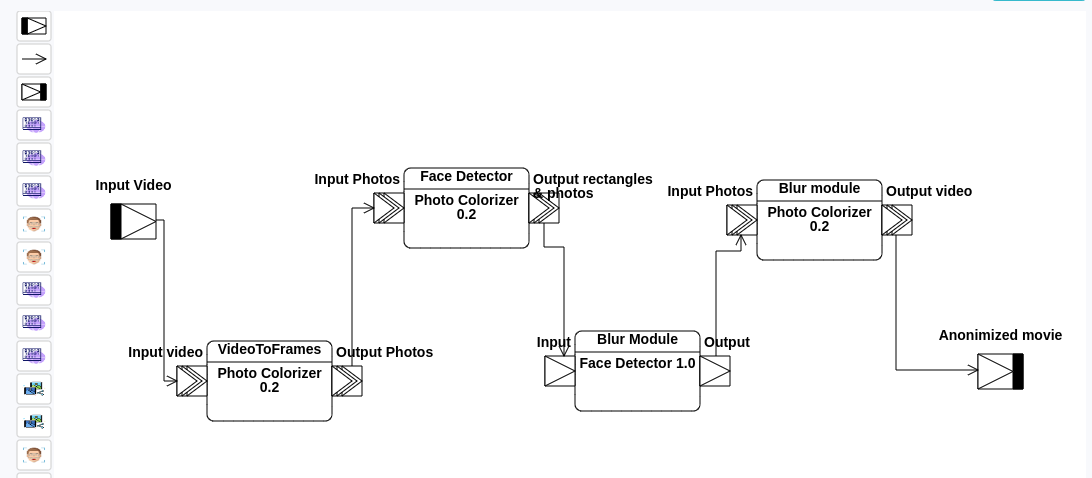
\includegraphics[width=0.95\linewidth]{./images/balticlsc-example-diagram.png}
	\caption{Aplikacja obliczeniowa w BalticLSC z obliczeniami
		sekwencyjnymi.}\label{rys:sekwencyjna-aplikacja-obliczeniowa}
\end{figure}

% \begin{noindent}
\begin{figure}[!ht]
	\centering

	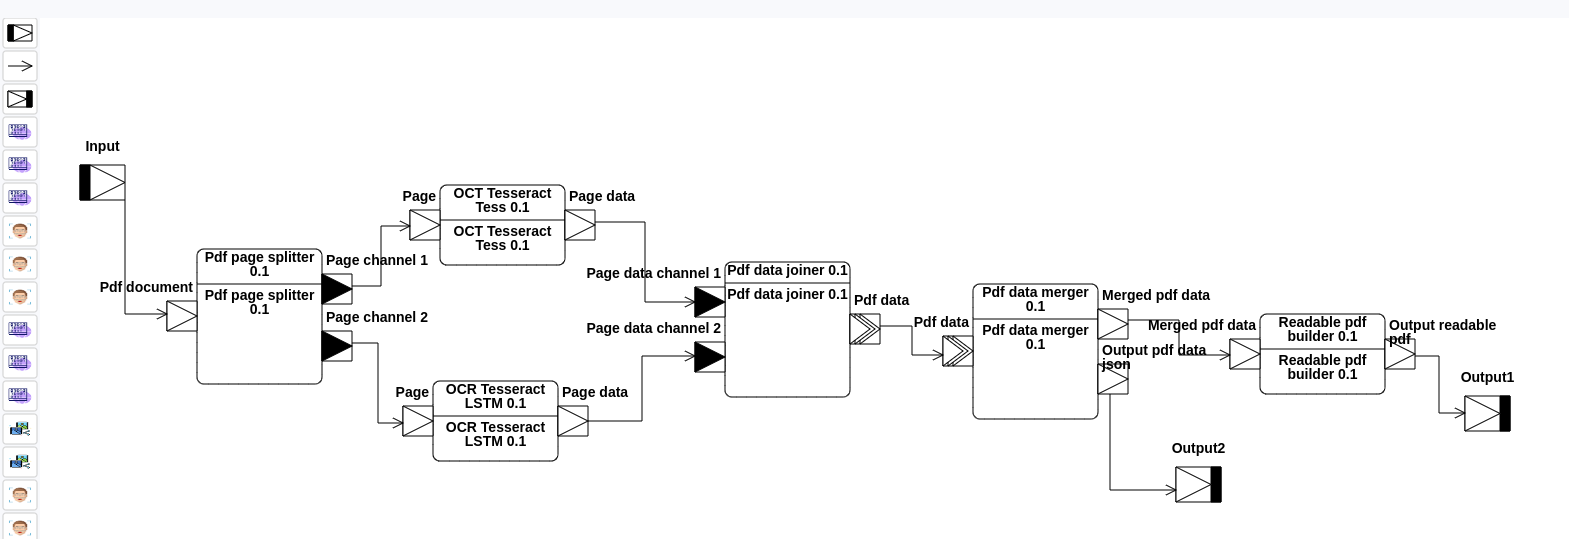
\includegraphics[width=0.99\linewidth]{./images/balticlsc-concurrent-application-example.png}
	\caption{Aplikacja obliczeniowa w BalticLSC z możliwością
		zrównoleglenia obliczeń.}\label{rys:mozliwa-do-zrownoleglenia-aplikacja-obliczeniowa}
\end{figure}
% \end{noindent}

\section{Stworzony metamodel EMF dla języka CAL}

Przygotowany metamodel \gls{EMF} dla języka \gls{CAL} widoczny jest na
rysunku~\ref{rys:cal-emf-metamodel}. Bazuje on~na metamodelu
opracowanym w ramach projektu BalticLSC~\cite{cal-metamodel}, który widoczny
jest na~rysunku~\ref{rys:cal-metamodel-balticlsc}.
Na potrzeby edytora diagramów nie są potrzebne wszystkie elementy oryginalnego
metamodelu. Niektóre klasy i właściwości zostały pominięte, ponieważ nie były
istotne z~perspektywy edycji diagramu.

\begin{figure}[!hb]
	\centering

	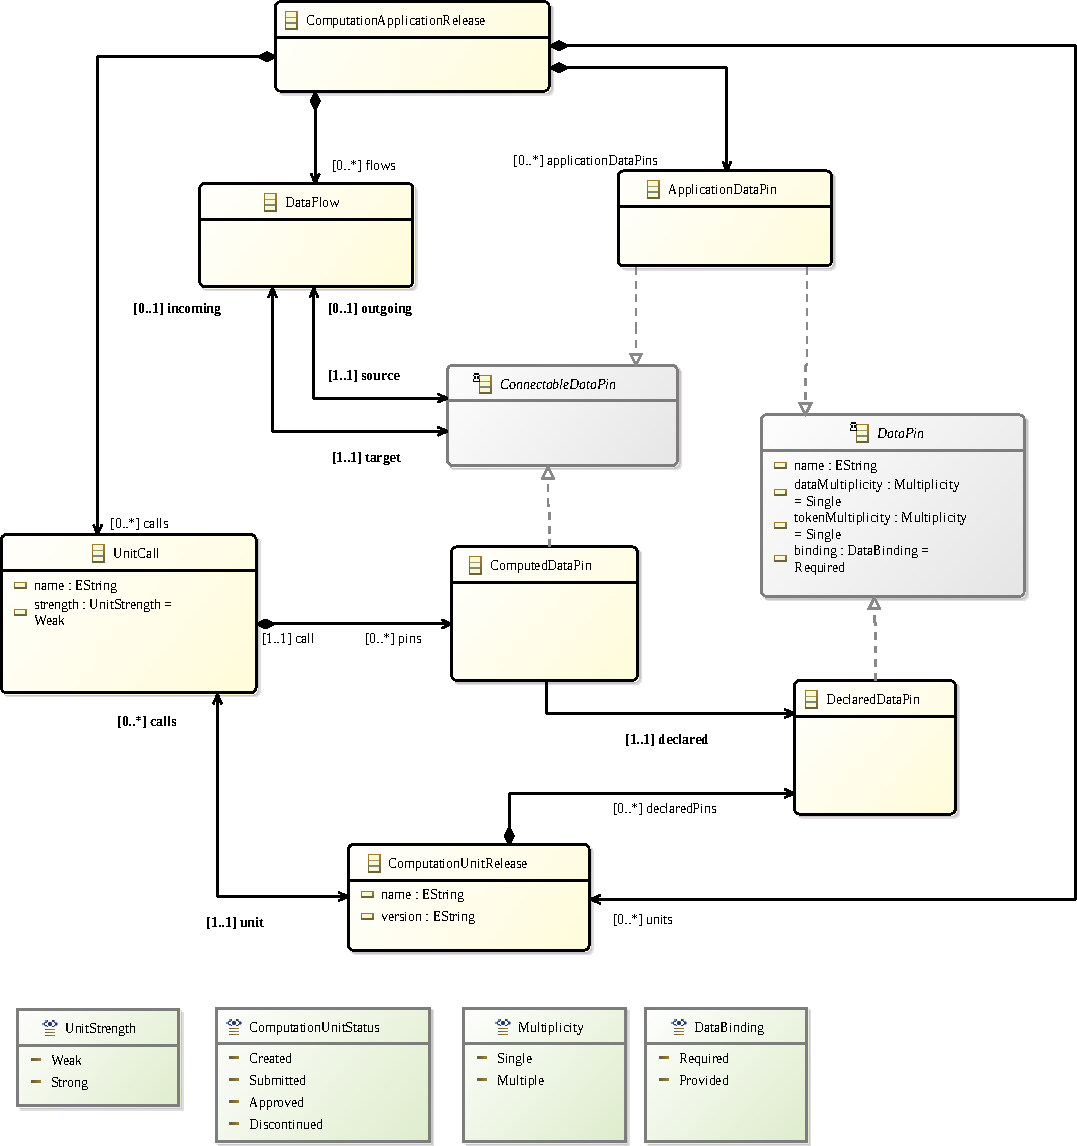
\includegraphics[width=0.92\linewidth]{./images/cal-emf-metamodel.pdf}
	\caption{Metamodel EMF języka CAL przygotowany w ramach tej
		pracy.}\label{rys:cal-emf-metamodel}
\end{figure}

\begin{figure}[!hb]
	\centering

	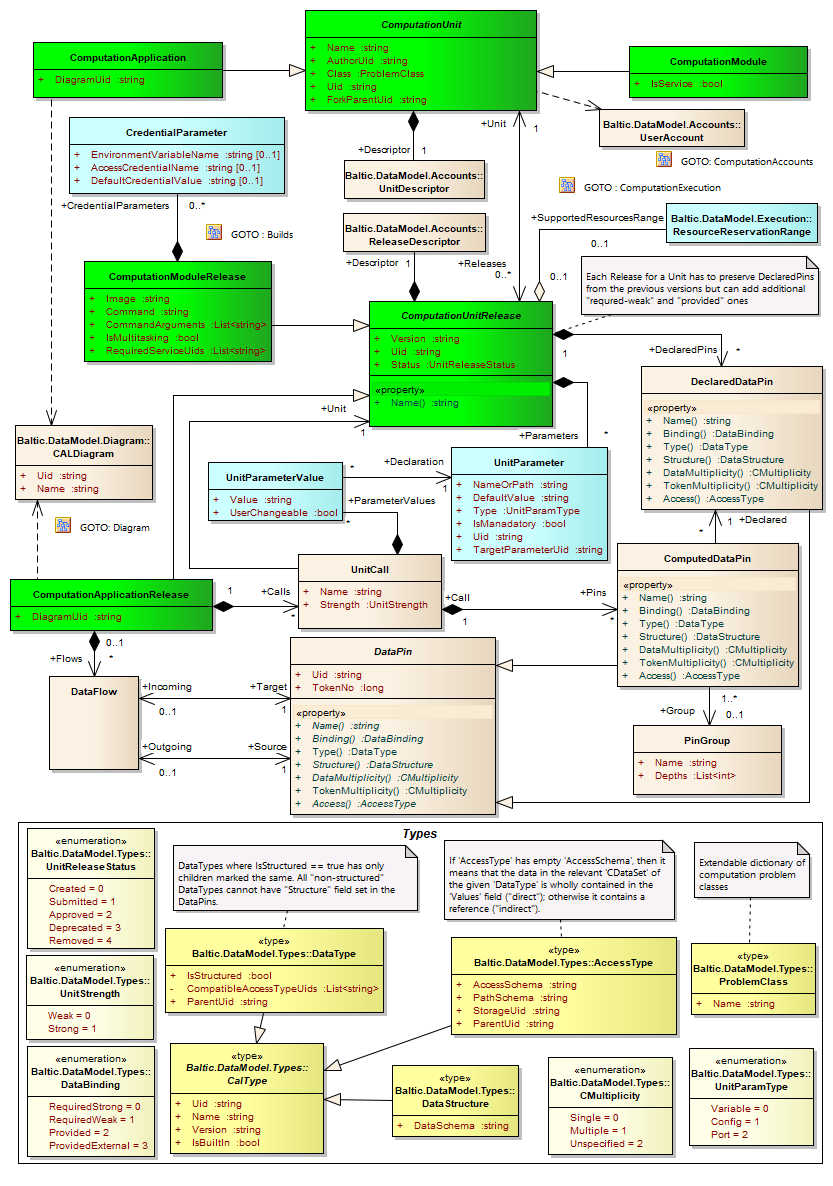
\includegraphics[width=0.92\linewidth]{./images/cal-metamodel-balticlsc.png}
	\caption{Metamodel języka CAL używany w projekcie
		BalticLSC\@.}\label{rys:cal-metamodel-balticlsc}

	\medskip
	{\small Źródło:
		\url{https://www.balticlsc.eu/model/index.htm?goto=4:2:404}}
\end{figure}

Model w EMF jest strukturą drzewiastą. Korzeniem drzewa jest obiekt typu
\texttt{ComputationApplicationRelease}, ktory odpowiada całemu diagramowi. Nie
ma on~własnych właściwości. Zawiera on w sobie natomiast 4 typy obiektów:

\begin{itemize}
	\item \texttt{ComputationUnitRelease} --- są to obiekty odpowiadające
	      rodzajom modułów obliczeniowych dostępnych w systemie BalticLSC i opisują ich właściwości.

	      Oprócz informacji o nazwie i wersji modułu zawierają w sobie obiekty \texttt{DeclaredDataPin} dziedziczące z \texttt{DataPin}, które opisują porty tego modułu obliczeniowego.

	      Obiekty te nie są wyświetlane na diagramie (nie występują w wizualnej reprezentacji modelu). Można je zobaczyć jedynie w drzewie obiektów modelu.

	\item \texttt{UnitCall} --- wywołania dostępnych modułów
	      obliczeniowych. Każdy dostępny moduł obliczeniowy może zostać wywołany dowolną liczbę razy. Każde wywołanie to osobny obiekt \texttt{UnitCall} ze wskazaniem modułu, który ma zostać wywołany, a także z obiektami \texttt{ComputedDataPin}, które reprezentują porty tego modułu.

	      Taka reprezentacja pozwala na zapisanie szczegółów dotyczących dostępnych modułow obliczeniowych wyłącznie raz w modelu, a później wskazywaniu tych elementów w~każdym z wywołań modułu.

	      Rozwiązanie to ma jednak pewne ograniczenie --- aby oznaczyć wywołanie modułu za~pomocą obiektu \texttt{UnitCall}, należy najpierw stworzyć obiekt \texttt{ComputationUnitRelease} i~dodać odpowiednie \texttt{DeclaredDataPin}. Można wywołać jedynie moduły, które są~zapisane w metamodelu. Sam metamodel nie ma możliwości pobrania informacji o~dostępnych modułach obliczeniowych z systemu BalticLSC, więc w podstawowej wersji metamodelu to użytkownik musi samemu dodać dostępne moduły w metamodelu.

	      Na diagramie obiekty te są reprezentowane jako prostokąty ze swoimi portami umieszczonymi na krawędziach. Wewnątrz prostokąta znajduje się etykieta zawierająca nazwę umożliwiającą wyróżnienie tego konkretnego wywołania modułu, oraz nazwę i wersję wydania wywolywanego modułu.

	\item \texttt{ApplicationDataPin} --- porty aplikacji obliczeniowej
	      opisywanej przez ten model. Są~to~wejścia i wyjścia z diagramu. Właściwości portu są dziedziczone z klasy \texttt{DataPin}.

	      Z uwagi na fakt, że te porty będą łączone z innymi portami, klasa ta dziedziczy z klasy \texttt{ConnectableDataPin}.

	      Na diagramie obiekty te reprezentowane są jako prostokąty z ikoną strzałki w prawo z~pogrubionym prawym lub lewym jej bokiem.

	\item \texttt{DataFlow} --- połączenia między portami
	      (\texttt{ConnectableDataPin}) umieszczonymi na~wywołaniach węzłów
	      obliczeniowych (\texttt{ComputedDataPin} na \texttt{UnitCall}) lub portami aplikacji obliczeniowej (\texttt{ApplicationDataPin}).

	      Na diagramie obiekty te reprezentowane są jako krawędzie z grotem wskazującym kierunek przepływu danych.
\end{itemize}

Przykładowy diagram reprezentujący model EMF języka CAL wyświetlony w programie
\emph{Sirius Desktop} został przedstawione na
rysunku~\ref{rys:sirius-desktop-cal-example-model}.

% \begin{noindent}
\begin{figure}[!hb]
	\centering

	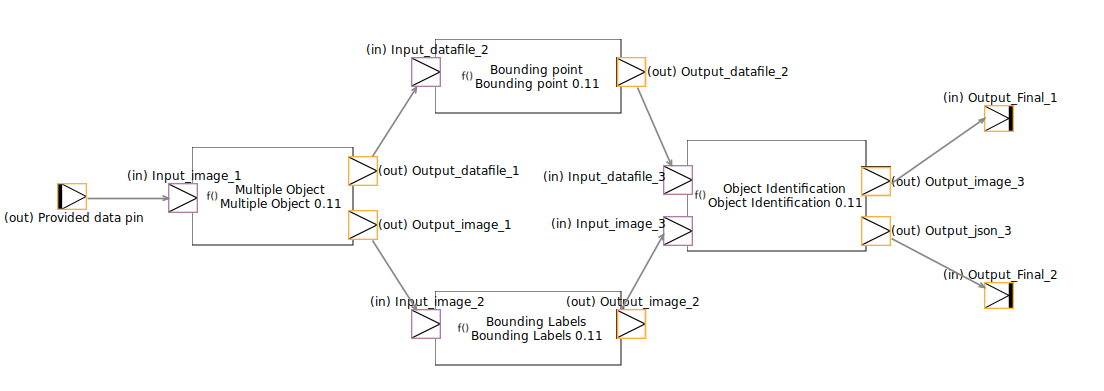
\includegraphics[width=0.95\linewidth]{./images/sirius-desktop-cal-example-model.png}
	\caption{Przykładowy diagram reprezentujący model EMF języka CAL w
		\emph{Sirius Desktop}.}\label{rys:sirius-desktop-cal-example-model}
\end{figure}
% \end{noindent}

Oprócz podstawowej struktury metamodelu oraz jego reprezentacji w formie
diagramu zostały do niego dodane dodatkowe funkcjonalności. Zostały one opisane
w kolejnych sekcjach.

\subsection{Warunkowa zmiana stylu elementów}

% \begin{noindent}
Użytkownik może wywnioskować dodatkowe informacje z diagramu jeżeli jego wygląd
będzie zależał od właściwości elementów modelu. Takie rozwiązanie zastosowano
dla dwóch elementów metamodelu dzięki wykorzystaniu \emph{Style
	Customizations}~\cite{sirius-desktop-documentation-style-customizations}
w \gls{EMF}.
% \end{noindent}
Funkcjonalność ta pozwala na wskazanie za pomocą języka \gls{AQL} w jakich
sytuacjach styl elementu powinien zostać zmieniony, a następnie wskazać które
właściwości powinny ulec zmianie oraz ich nowe wartości.

Pierwszym styl warunkowy został użyty dla portów w metamodelu. Porty
(\texttt{DataPin}) zmieniają ikonę na podstawie swoich krotności danych oraz
paczek danych (odpowiednio \emph{data multiplicity} i \emph{token
	multiplicity}).

Z uwagi na fakt, że oba parametry mogą mieć jedną z 2 wartości,
co daje w sumie 4~możliwości, w klasie \texttt{Services} metamodelu stworzono
metodę w języku Java, która zwraca nazwę odpowiedniej ikony.
Dzięki możliwości wykorzystania języka programowania osiągnięto
zamierzony efekt za pomocą jednego stylu warunkowego, a nie 4 różnych
styli dla 4 możliwości. Kod metody zwracającej nazwę ikony dla portu
został przedstawiony w listingu~\ref{lst:getDataPinIconPath-method}.

\begin{lstlisting}[language=Java,
    caption={Methoda zwracająca nazwę ikony dla portu.},
    label={lst:getDataPinIconPath-method}]
public String getDataPinIconPath(EObject self) {
  if (!(self instanceof DataPin)) {
    return null;
  }

  var dataPin = (DataPin) self;
  var dataPart = dataPin.getDataMultiplicity() == Multiplicity.SINGLE ? "single-data" : "multiple-data";
  var tokenPart = dataPin.getTokenMultiplicity() == Multiplicity.SINGLE ? "single-token" : "multiple-tokens";

  return dataPart + "-" + tokenPart + ".png";
}
\end{lstlisting}

Dla portów całej aplikacji obliczeniowej (\texttt{ApplicationDataPin} dla
\texttt{ComputationApplicationRelease}) styl warunkowy był rozszerzeniem tego
dla portów modułów obliczeniowych. Oprócz brania pod uwagę kroności danych oraz
paczek danych, w tym stylu znaczenie ma ponadto kierunek portu. Porty wejściowe
mają pogrubiony pasek z lewej strony, a porty wyjściowe z prawej. Dla tych
portów występują 3 cechy od których zależy ikona, co oznacza 8 możliwości.
Dzięki wykorzystaniu metody z listingu~\ref{lst:getDataPinIconPath-method} oraz
języka \gls{AQL} ta funkcjonalność została zrealizowana za pomocą jednego stylu
warunkowego, zamiast 8 styli dla 8 różnych waruantow.

Drugim wykorzystanym rodzajem styli warunkowych jest zmiana koloru obramowania
portów na krawędziach modułów obliczeniowych (\texttt{ComputedDataPin}) w
zależności od~kierunku przepływu danych. Porty wejściowe (\emph{required}) mają
ramkę koloru fioletowego, a~porty wyjściowe (\emph{provided}) mają ramkę koloru
pomarańczowego. Ta funkcjonalność została zaimplementowana za pomocą jednego
stylu warunkowego.

Wyniki działania obu rodzajów styli warunkowych widoczne są na
rysunku~\ref{rys:sirius-desktop-cal-example-model}.

\subsection{Narzędzia edytora diagramów}

Omówienie dodanych \textit{Tools} z Sirius:

\begin{itemize}
	\item usunięcie \texttt{UnitCall} lub \texttt{ApplicationDataPin} usuwa również powiązane \texttt{DataFlow}
	\item usunięcie \texttt{ComputedDataPin} z poziomu edytora diagramów nie jest możliwe
	\item ograniczenia na tworzenie \texttt{DataFlow} tak, aby były semantycznie poprawne
	\item automatyczne usuwanie i tworzenie \texttt{ComputedDataPin} po zmianie \texttt{ComputationUnitRelease} dla danego \texttt{UnitCall}
	\item okno dialogowe ułatwiające tworzenie \texttt{UnitCall} dla istniejącego \texttt{ComputationUnitRelease}
	\item \ldots
\end{itemize}

\subsection{Reguły walidacyjne powiązane z
	metamodelem}\label{sec:regulky-walidacyjne-metamodel}

Omówienie \textit{semantic validation rule} z pliku \texttt{*.odesign}, które
działają w Sirius Desktop.

\subsection{Testy metamodelu}

Omówienie dodanych testów jednostkowych modelu (głównie dotyczy automatycznego
zarządzania \texttt{ComputedDataPin} w zależnosci od
\texttt{ComputationUnitRelease} dla konkretnego \texttt{UnitCall}).
